\documentclass[12pt,spanish]{article}
\usepackage[spanish]{babel}
\usepackage{graphicx}
\usepackage{subcaption}

\usepackage{multirow}
\usepackage{hyperref}
\usepackage{caption}
\usepackage{multicol}
\usepackage[outputdir=build]{minted}
\usepackage[skins,minted,breakable]{tcolorbox}
\usepackage{float}
\usepackage{array}
\graphicspath{ {../img/} {../../LaTeX/img/} {/home/csp98/latex/img/}}
\selectlanguage{spanish}
\usepackage[utf8]{inputenc}
\usepackage{graphicx}
\usepackage[a4paper,left=3cm,right=2cm,top=2.5cm,bottom=2.5cm]{geometry}
\newtheorem{ppio}{Principio }
\makeindex

\begin{document}
\begin{titlepage}

\newlength{\centeroffset}
\setlength{\centeroffset}{-0.5\oddsidemargin}
\addtolength{\centeroffset}{0.5\evensidemargin}
\thispagestyle{empty}

\noindent\hspace*{\centeroffset}
\begin{minipage}{\textwidth}

\centering
\includegraphics[width=0.9\textwidth]{logo_ugr.jpg}\\[1.4cm]

\textsc{ \Large Algorítmica\\[0.2cm]}
\textsc{GRADO EN INGENIERÍA INFORMÁTICA}\\[1cm]

{\Huge\bfseries Práctica 1\\}
\noindent\rule[-1ex]{\textwidth}{3pt}\\[3.5ex]
{\large\bfseries Análisis de eficiencia de algoritmos}
\end{minipage}

\vspace{1.5cm}
\noindent\hspace*{\centeroffset}
\begin{minipage}{\textwidth}
\centering

\textbf{Autores}\\ {Maria Jesús López Salmerón \\ Nazaret Román Guerrero \\ Laura Hernández Muñoz \\ José Baena Cobos  \\ Carlos Sánchez Páez}\\[2.5ex]
\includegraphics[width=0.3\textwidth]{etsiit_logo.png}\\[0.1cm]
\vspace{1.5cm}
\includegraphics[width=0.5\textwidth]{decsai.jpg}\\[0.1cm]
\vspace{1cm}
\textsc{Escuela Técnica Superior de Ingenierías Informática y de Telecomunicación}\\
\vspace{1cm}
\textsc{Curso 2017-2018}
\end{minipage}
\end{titlepage}
\tableofcontents
\thispagestyle{empty}
\listoftables
\newpage
\setcounter{page}{1}
%%%%%%%%%%%%%%%%%%%%%%%%Comienzo del documento%%%%%%%%%%%%%%%%%%%%%%%%%%%%%%%
\section{Descripción de la práctica}

El objetivo de la práctica es analizar la eficiencia de distintos algoritmos mediante dos métodos:
\begin{enumerate}
\item \textbf{Empírico}: ejecutando dicho algoritmo con distintos tamaños de problema y analizando el tiempo de realización del mismo frente a la cantidad de datos de entrada.
\item \textbf{Híbrido}: Hayando las constantes ocultas en la expresión \textit{T(n)} mediante los datos empíricos obtenidos anteriormente.
\end{enumerate}
\section{Código fuente a utilizar}

Los algoritmos que utilizaremos para realizar la práctica han sido descargados de la plataforma \textit{decsai.ugr.es}.

\subsection{Hanoi}
\begin{multicols}{2}
\begin{tcblisting}{
  enhanced,
  listing only,
  minted options={
    baselinestretch=1.0,
    %bgcolor=lightgray,
    fontsize=\footnotesize,
    linenos,
    breaklines,
  },
  minted language=c++,
  boxrule=0pt,
  boxsep=0pt,
  frame hidden,
  breakable=unlimited,
}  
#include <iostream>
using namespace std;
#include <ctime>
#include <cstdlib>

/**
   @brief Resuelve el problema de las Torres de Hanoi
   @param M: número de discos. M > 1.
   @param i: número de columna en que están los discos.
             i es un valor de {1, 2, 3}. i != j.
   @param j: número de columna a que se llevan los discos.
             j es un valor de {1, 2, 3}. j != i.

   Esta función imprime en la salida estándar la secuencia de 
   movimientos necesarios para desplazar los M discos de la
   columna i a la j, observando la restricción de que ningún
   disco se puede situar sobre otro de tamaño menor. Utiliza
   una única columna auxiliar.
*/
void hanoi (int M, int i, int j);

void hanoi (int M, int i, int j)
{
  if (M > 0)
    {
      hanoi(M-1, i, 6-i-j);
      cout << i << " -> " << j << endl;
      hanoi (M-1, 6-i-j, j);
  }
}

int main(int argc, char * argv[])
{
  
    if (argc != 2)
    {
      cerr << "Formato " << argv[0] << " <num_discos>" << endl;
      return -1;
    }

  int M = atoi(argv[1]);

  clock_t tantes;    // Valor del reloj antes de la ejecución
  clock_t tdespues;  // Valor del reloj después de la ejecución
  tantes = clock();
  hanoi(M, 1, 2);
  tdespues = clock();
  cout << M << 
  ((double)(tdespues-tantes))
  /CLOCKS_PER_SEC << endl; 
  return 0;
}
\end{tcblisting}
\end{multicols}
\newpage

\subsection{Floyd}
\begin{multicols}{2}
\begin{tcblisting}
{
  enhanced,
  listing only,
  minted options={
    baselinestretch=1.0,
    fontsize=\footnotesize,
    linenos,
    breaklines,
  },
  minted language=c++,
  boxrule=0pt,
  boxsep=0pt,
  frame hidden,
  breakable=unlimited,
}
  
#include <iostream>
using namespace std;
#include <ctime>
#include <cstdlib>
#include <climits>
#include <cassert>
#include <cmath>

static int const MAX_LONG  = 10;
            
/**
   @brief Reserva espacio en memoria dinámica para una matriz cuadrada.
   
   @param dim: dimensión de la matriz. dim > 0.

   @returns puntero a la zona de memoria reservada.
*/
int ** ReservaMatriz(int dim);

/**
   @brief Libera el espacio asignado a una matriz cuadrada.
   
   @param M: puntero a la zona de memoria reservada. Es MODIFICADO.
   @param dim: dimensión de la matriz. dim > 0.

   Liberar la zona memoria asignada a M y lo pone a NULL.
*/
void LiberaMatriz(int ** & M, int dim);

/**
   @brief Rellena una matriz cuadrada con valores aleaotorias.
   
   @param M: puntero a la zona de memoria reservada. Es MODIFICADO.
   @param dim: dimensión de la matriz. dim > 0.

   Asigna un valor aleatorio entero de [0, MAX_LONG - 1] a cada
   elemento de la matriz M, salvo los de la diagonal principal
   que quedan a 0..
*/
void RellenaMatriz(int **M, int dim);

/**
   @brief Cálculo de caminos mínimos.
   
   @param M: Matriz de longitudes de los caminos. Es MODIFICADO.
   @param dim: dimensión de la matriz. dim > 0.

   Calcula la longitud del camino mínimo entre cada par de nodos (i,j),
   que se almacena en M[i][j].
*/
void Floyd(int **M, int dim);


/**
   Implementación de las funciones
**/

int ** ReservaMatriz(int dim)
{
  int **M;
  if (dim  <= 0)
    {
      cerr<< "\n ERROR: Dimension de la matriz debe ser mayor que 0" << endl;
      exit(1);
    }
  M = new int * [dim];
  if (M == NULL)
    {
      cerr << "\n ERROR: No puedo reservar memoria para un matriz de "
	   << dim << " x " << dim << "elementos" << endl;
      exit(1);
    }
  for (int i = 0; i < dim; i++)
    {
      M[i]= new int [dim];
      if (M[i] == NULL)
	{
	  cerr << "ERROR: No puedo reservar memoria para un matriz de "
	       << dim << " x " << dim << endl;
	  for (int j = 0; j < i; j++)
	    delete [] M[i];
	  delete [] M;
	  exit(1);
	} 
    }
  return M;
}	

void LiberaMatriz(int ** & M, int dim)
{
  for (int i = 0; i < dim; i++)
    delete [] M[i];
  delete [] M;
  M = NULL;
}		


void RellenaMatriz(int **M, int dim)
{
  for (int i = 0; i < dim; i++)
    for (int j = 0; j < dim; j++)
      if (i != j)
	M[i][j]= (rand() \% MAX_LONG);
}			
	
void Floyd(int **M, int dim)
{
	for (int k = 0; k < dim; k++)
	  for (int i = 0; i < dim;i++)
	    for (int j = 0; j < dim;j++)
	      {
		int sum = M[i][k] + M[k][j];    	
	    	M[i][j] = (M[i][j] > sum) ? sum : M[i][j];
	      }
}	     	

int main (int argc, char **argv)
{
//  clock_t tantes;   
//  clock_t tdespues;
    int dim;          

  //Lectura de los parametros de entrada
  if (argc != 2)
    {
      cout << "Parámetros de entrada: " << endl
	   << "1.- Número de nodos" << endl << endl;
      return 1;	
    }	

  dim = atoi(argv[1]);	
  int ** M = ReservaMatriz(dim);

  RellenaMatriz(M,dim);
		
			
 // Empieza el algoritmo de floyd
  tantes = clock();
  Floyd(M,dim);
  tdespues = clock();
  cout << dim  << 
  ((double)(tdespues-tantes))
  /CLOCKS_PER_SEC << endl;
  LiberaMatriz(M,dim);

  return 0;	
\end{tcblisting}
\end{multicols}
\newpage

\subsection{Algoritmos de ordenación}

\subsubsection{Burbuja}

\begin{multicols}{2}
\begin{tcblisting}
{
  enhanced,
  listing only,
  minted options={
    baselinestretch=1.0,
    %bgcolor=lightgray,
    fontsize=\footnotesize,
    linenos,
    breaklines,
  },
  minted language=c++,
  boxrule=0pt,
  boxsep=0pt,
  frame hidden,
  breakable=unlimited,
}

#include <iostream>
using namespace std;
#include <ctime>
#include <cstdlib>
#include <climits>
#include <cassert>

/**
   @brief Ordena un vector por el método de la burbuja.

   @param T: vector de elementos. Debe tener num_elem elementos.
             Es MODIFICADO.
   @param num_elem: número de elementos. num_elem > 0.

   Cambia el orden de los elementos de T de forma que los dispone
   en sentido creciente de menor a mayor.
   Aplica el algoritmo de la burbuja.
*/
inline static 
void burbuja(int T[], int num_elem);

/**
   @brief Ordena parte de un vector por el método de la burbuja.

   @param T: vector de elementos. Tiene un número de elementos 
                   mayor o igual a final.Es MODIFICADO.

   @param inicial: Posición que marca el incio de la parte del
                   vector a ordenar.
   @param final: Posición detrás de la última de la parte del
                   vector a ordenar. 
		   inicial < final.

   Cambia el orden de los elementos de T entre las posiciones
   inicial y final - 1de forma que los dispone en sentido creciente
   de menor a mayor.
   Aplica el algoritmo de la burbuja.
*/
static void burbuja_lims(int T[], int inicial, int final);

/**
   Implementación de las funciones
**/

inline void burbuja(int T[], int num_elem)
{
  burbuja_lims(T, 0, num_elem);
}

static void burbuja_lims(int T[], int inicial, int final)
{
  int i, j;
  int aux;
  for (i = inicial; i < final - 1; i++)
    for (j = final - 1; j > i; j--)
      if (T[j] < T[j-1])
	{
	  aux = T[j];
	  T[j] = T[j-1];
	  T[j-1] = aux;
	}
}

int main(int argc, char * argv[]){
    if (argc != 2){
      cerr << "Formato " << argv[0] << " <num_elem>" << endl;
      return -1;
    }
  int n = atoi(argv[1]);
  int * T = new int[n];
  assert(T);
  srandom(time(0));

  for (int i = 0; i < n; i++)
      T[i] = random();

  clock_t tantes;  
  clock_t tdespues; 
  tantes = clock();
  burbuja(T, n);
  tdespues = clock();
  cout << n  << 
  ((double)(tdespues-tantes))
  /CLOCKS_PER_SEC << endl;
  
  delete [] T;

  return 0;
}
\end{tcblisting}
\end{multicols}
\newpage
\subsubsection{Selección}
\begin{multicols}{2}
\begin{tcblisting}
{
  enhanced,
  listing only,
  minted options={
    baselinestretch=1.0,
    %bgcolor=lightgray,
    fontsize=\footnotesize,
    linenos,
    breaklines,
  },
  minted language=c++,
  boxrule=0pt,
  boxsep=0pt,
  frame hidden,
  breakable=unlimited,
}
#include <iostream>
using namespace std;
#include <ctime>
#include <cstdlib>
#include <climits>
#include <cassert>

/**
   @brief Ordena un vector por el método de selección.

   @param T: vector de elementos. Debe tener num_elem elementos.
             Es MODIFICADO.
   @param num_elem: número de elementos. num_elem > 0.

   Cambia el orden de los elementos de T de forma que los dispone
   en sentido creciente de menor a mayor. Aplica el algoritmo de selección.
*/
inline static 
void seleccion(int T[], int num_elem);

/**
   @brief Ordena parte de un vector por el método de selección.

   @param T: vector de elementos. Tiene un número de elementos 
                   mayor o igual a final. Es MODIFICADO.
   @param inicial: Posición que marca el incio de la parte del
                   vector a ordenar.
   @param final: Posición detrás de la última de la parte del
                   vector a ordenar. 
		   inicial < final.

   Cambia el orden de los elementos de T entre las posiciones
   inicial y final - 1de forma que los dispone en sentido creciente
   de menor a mayor. Aplica el algoritmo de selección.
*/
static void seleccion_lims(int T[], int inicial, int final);
/**
   Implementación de las funciones
**/

void seleccion(int T[], int num_elem){
  seleccion_lims(T, 0, num_elem);
}

static void seleccion_lims(int T[], int inicial, int final){
  int i, j, indice_menor;
  int menor, aux;
  for (i = inicial; i < final - 1; i++) {
    indice_menor = i;
    menor = T[i];
    for (j = i; j < final; j++)
      if (T[j] < menor) {
	indice_menor = j;
	menor = T[j];
      }
    aux = T[i];
    T[i] = T[indice_menor];
    T[indice_menor] = aux;
  }
}

int main(int argc, char * argv[]){
  if (argc != 2){
      cerr << "Formato " << argv[0] << " <num_elem>" << endl;
      return -1;
   }
  int n = atoi(argv[1]);
  int * T = new int[n];
  assert(T);
  srandom(time(0));

  for (int i = 0; i < n; i++)
      T[i] = random();

  clock_t tantes;    // Valor del reloj antes de la ejecución
  clock_t tdespues;  // Valor del reloj después de la ejecución
  tantes = clock();
  seleccion(T, n);
  tdespues = clock();
  cout << n << ((double)(tdespues-tantes))
  /CLOCKS_PER_SEC << endl;
  
  delete [] T;
  return 0;
}
\end{tcblisting}
\end{multicols}
\newpage
\subsubsection{Inserción}
\begin{multicols}{2}
\begin{tcblisting}
{
  enhanced,
  listing only,
  minted options={
    baselinestretch=1.0,
    %bgcolor=lightgray,
    fontsize=\footnotesize,
    linenos,
    breaklines,
  },
  minted language=c++,
  boxrule=0pt,
  boxsep=0pt,
  frame hidden,
  breakable=unlimited,
}
#include <iostream>
using namespace std;
#include <ctime>
#include <cstdlib>
#include <climits>
#include <cassert>

/**
   @brief Ordena un vector por el método de inserción.

   @param T: vector de elementos. Debe tener num_elem elementos.
             Es MODIFICADO.
   @param num_elem: número de elementos. num_elem > 0.

   Cambia el orden de los elementos de T de forma que los dispone
   en sentido creciente de menor a mayor.
   Aplica el algoritmo de inserción.
*/
inline static 
void insercion(int T[], int num_elem);

/**
   @brief Ordena parte de un vector por el método de inserción.

   @param T: vector de elementos. Tiene un número de elementos 
                   mayor o igual a final. Es MODIFICADO.
   @param inicial: Posición que marca el incio de la parte del
                   vector a ordenar.
   @param final: Posición detrás de la última de la parte del
                   vector a ordenar. 
		   inicial < final.

   Cambia el orden de los elementos de T entre las posiciones
   inicial y final - 1de forma que los dispone en sentido creciente
   de menor a mayor.
   Aplica el algoritmo de inserción.
*/
static void insercion_lims(int T[], int inicial, int final);

/**
   Implementación de las funciones
**/

inline static void insercion(int T[], int num_elem){
  insercion_lims(T, 0, num_elem);
}

static void insercion_lims(int T[], int inicial, int final){
  int i, j;
  int aux;
  for (i = inicial + 1; i < final; i++) {
    j = i;
    while ((T[j] < T[j-1]) && (j > 0)) {
      aux = T[j];
      T[j] = T[j-1];
      T[j-1] = aux;
      j--;
    };
  };
}

int main(int argc, char * argv[]){ 
    if (argc != 2){
      cerr << "Formato " << argv[0] << " <num_elem>" << endl;
      return -1;
    }
  int n = atoi(argv[1]);

  int * T = new int[n];
  assert(T);

  srandom(time(0));

  for (int i = 0; i < n; i++)
      T[i] = random();

  clock_t tantes;    // Valor del reloj antes de la ejecución
  clock_t tdespues;  // Valor del reloj después de la ejecución
  tantes = clock();
  insercion(T, n);
  tdespues = clock();
  cout << n << ((double)(tdespues-tantes))
  /CLOCKS_PER_SEC << endl;
  delete [] T;

  return 0;
};
\end{tcblisting}
\end{multicols}
\newpage
\subsubsection{\textit{Heapsort}}

\begin{multicols}{2}
\begin{tcblisting}
{
  enhanced,
  listing only,
  minted options={
    baselinestretch=1.0,
    %bgcolor=lightgray,
    fontsize=\footnotesize,
    linenos,
    breaklines,
  },
  minted language=c++,
  boxrule=0pt,
  boxsep=0pt,
  frame hidden,
  breakable=unlimited,
}   
#include <iostream>
using namespace std;
#include <ctime>
#include <cstdlib>
#include <climits>
#include <cassert>

/**
   @brief Ordena un vector por el método de montones.

   @param T: vector de elementos. Debe tener num_elem elementos.Es MODIFICADO.
   @param num_elem: número de elementos. num_elem > 0.

   Cambia el orden de los elementos de T de forma que los dispone
   en sentido creciente de menor a mayor.Aplica el algoritmo de ordenación por montones.
*/
inline static 
void heapsort(int T[], int num_elem);

/**
   @brief Reajusta parte de un vector para que sea un montón.

   @param T: vector de elementos. Debe tener num_elem elementos.
             Es MODIFICADO.
   @param num_elem: número de elementos. num_elem > 0.
   @param k: índice del elemento que se toma com raíz
   
   Reajusta los elementos entre las posiciones k y num_elem - 1 
   de T para que cumpla la propiedad de un montón (APO), 
   considerando al elemento en la posición k como la raíz.
*/
static void reajustar(int T[], int num_elem, int k);

/**Implementación de las funciones**/

static void heapsort(int T[], int num_elem){
  int i;
  for (i = num_elem/2; i >= 0; i--)
    reajustar(T, num_elem, i);
  for (i = num_elem - 1; i >= 1; i--){
      int aux = T[0];
      T[0] = T[i];
      T[i] = aux;
      reajustar(T, i, 0);
    }
}
  
static void reajustar(int T[], int num_elem, int k){
  int j;
  int v;
  v = T[k];
  bool esAPO = false;
  while ((k < num_elem/2) && !esAPO)
    {
      j = k + k + 1;
      if ((j < (num_elem - 1)) && (T[j] < T[j+1]))
	j++;
      if (v >= T[j])
	esAPO = true;
      T[k] = T[j];
      k = j;
    }
  T[k] = v;
}
       
int main(int argc, char * argv[]){
  if (argc != 2){
      cerr << "Formato " << argv[0] << " <num_elem>" << endl;
      return -1;
   }
  int n = atoi(argv[1]);
  int * T = new int[n];
  assert(T);
  srandom(time(0));
  for (int i = 0; i < n; i++)
      T[i] = random();

  clock_t tantes;    // Valor del reloj antes de la ejecución
  clock_t tdespues;  // Valor del reloj después de la ejecución
  tantes = clock();
  heapsort(T, n);
  tdespues = clock();
  cout << n << ((double)(tdespues-tantes))
  /CLOCKS_PER_SEC << endl;

  delete [] T;
  return 0;
};
\end{tcblisting}
\end{multicols}
\newpage
\subsubsection{\textit{Mergesort}}

\begin{multicols}{2}
\begin{tcblisting}
{
  enhanced,
  listing only,
  minted options={
    baselinestretch=1.0,
    %bgcolor=lightgray,
    fontsize=\footnotesize,
    linenos,
    breaklines,
  },
  minted language=c++,
  boxrule=0pt,
  boxsep=0pt,
  frame hidden,
  breakable=unlimited,
} 
#include <iostream>
using namespace std;
#include <ctime>
#include <cstdlib>
#include <climits>
#include <cassert>
/**
   @brief Ordena un vector por el método de mezcla.

   @param T: vector de elementos. Debe tener num_elem elementos.
             Es MODIFICADO.
   @param num_elem: número de elementos. num_elem > 0.

   Cambia el orden de los elementos de T de forma que los dispone
   en sentido creciente de menor a mayor. Aplica el algoritmo de mezcla.
*/
inline static 
void mergesort(int T[], int num_elem);
/**
   @brief Ordena parte de un vector por el método de mezcla.

   @param T: vector de elementos. Tiene un número de elementos 
                   mayor o igual a final. Es MODIFICADO.
   @param inicial: Posición que marca el incio de la parte del
                   vector a ordenar.
   @param final: Posición detrás de la última de la parte del
                   vector a ordenar. 
		   inicial < final.

   Cambia el orden de los elementos de T entre las posiciones
   inicial y final - 1 de forma que los dispone en sentido creciente
   de menor a mayor. Aplica el algoritmo de la mezcla.
*/
static void mergesort_lims(int T[], int inicial, int final);
/**
   @brief Ordena un vector por el método de inserción.

   @param T: vector de elementos. Debe tener num_elem elementos.
             Es MODIFICADO.
   @param num_elem: número de elementos. num_elem > 0.

   Cambia el orden de los elementos de T de forma que los dispone
   en sentido creciente de menor a mayor. Aplica el algoritmo de inserción.
*/
inline static 
void insercion(int T[], int num_elem);
/**
   @brief Ordena parte de un vector por el método de inserción.

   @param T: vector de elementos. Tiene un número de elementos 
                   mayor o igual a final. Es MODIFICADO.
   @param inicial: Posición que marca el incio de la parte del
                   vector a ordenar.
   @param final: Posición detrás de la última de la parte del
                   vector a ordenar. inicial < final.
   Cambia el orden de los elementos de T entre las posiciones
   inicial y final - 1 de forma que los dispone en sentido creciente
   de menor a mayor. Aplica el algoritmo de la inserción.
*/
static void insercion_lims(int T[], int inicial, int final);
/**
   @brief Mezcla dos vectores ordenados sobre otro.

   @param T: vector de elementos. Tiene un número de elementos 
                   mayor o igual a final. Es MODIFICADO.
   @param inicial: Posición que marca el incio de la parte del
                   vector a escribir.
   @param final: Posición detrás de la última de la parte del
                   vector a escribir
		   inicial < final.
   @param U: Vector con los elementos ordenados.
   @param V: Vector con los elementos ordenados.
             El número de elementos de U y V sumados debe coincidir
             con final - inicial.

   En los elementos de T entre las posiciones inicial y final - 1
   pone ordenados en sentido creciente, de menor a mayor, los
   elementos de los vectores U y V.
*/
static void fusion(int T[], int inicial, int final, int U[], int V[]);
/**
   Implementación de las funciones
**/
inline static void insercion(int T[], int num_elem){
  insercion_lims(T, 0, num_elem);
}
static void insercion_lims(int T[], int inicial, int final){
  int i, j;
  int aux;
  for (i = inicial + 1; i < final; i++) {
    j = i;
    while ((T[j] < T[j-1]) && (j > 0)) {
      aux = T[j];
      T[j] = T[j-1];
      T[j-1] = aux;
      j--;
    };
  };
}
const int UMBRAL_MS = 100;
void mergesort(int T[], int num_elem){
  mergesort_lims(T, 0, num_elem);
}
static void mergesort_lims(int T[], int inicial, int final){
  if (final - inicial < UMBRAL_MS)
      insercion_lims(T, inicial, final);
  else {
      int k = (final - inicial)/2;
      int * U = new int [k - inicial + 1];
      assert(U);
      int l, l2;
      for (l = 0, l2 = inicial; l < k; l++, l2++)
		U[l] = T[l2];
      U[l] = INT_MAX;
      int * V = new int [final - k + 1];
      assert(V);
      for (l = 0, l2 = k; l < final - k; l++, l2++)
		V[l] = T[l2];
      V[l] = INT_MAX;

      mergesort_lims(U, 0, k);
      mergesort_lims(V, 0, final - k);
      fusion(T, inicial, final, U, V);
      delete [] U;
      delete [] V;
    };
}
  
static void fusion(int T[], int inicial, int final, int U[], int V[]){
  int j = 0;
  int k = 0;
  for (int i = inicial; i < final; i++)
      if (U[j] < V[k]) {
		T[i] = U[j];j++;
      } else{
		T[i] = V[k];k++;
      }
}
int main(int argc, char * argv[]){
  if (argc != 2){
      cerr << "Formato " << argv[0] << " <num_elem>" << endl;
      return -1;
    }
  int n = atoi(argv[1]);
  int * T = new int[n];
  assert(T);
  srandom(time(0));
  for (int i = 0; i < n; i++)
      T[i] = random();
      
  clock_t tantes;    // Valor del reloj antes de la ejecución
  clock_t tdespues;  // Valor del reloj después de la ejecución
  tantes = clock();
  mergesort(T, n);
  tdespues = clock();
  cout << n << ((double)(tdespues-tantes))
  /CLOCKS_PER_SEC << endl;
  delete [] T;
  return 0;
};
\end{tcblisting}
\end{multicols}
\newpage
\subsubsection{\textit{Quicksort}}

\begin{multicols}{2}
\begin{tcblisting}
{
  enhanced,
  listing only,
  minted options={
    baselinestretch=1.0,
    %bgcolor=lightgray,
    fontsize=\footnotesize,
    linenos,
    breaklines,
  },
  minted language=c++,
  boxrule=0pt,
  boxsep=0pt,
  frame hidden,
  breakable=unlimited,
}
#include <iostream>
using namespace std;
#include <ctime>
#include <cstdlib>
#include <climits>
#include <cassert>
/**
   @brief Ordena un vector por el método quicksort.

   @param T: vector de elementos. Debe tener num_elem elementos.
             Es MODIFICADO.
   @param num_elem: número de elementos. num_elem > 0.

   Cambia el orden de los elementos de T de forma que los dispone
   en sentido creciente de menor a mayor.
   Aplica el algoritmo quicksort.
*/
inline static 
void quicksort(int T[], int num_elem);
/**
   @brief Ordena parte de un vector por el método quicksort.

   @param T: vector de elementos. Tiene un número de elementos 
                   mayor o igual a final. Es MODIFICADO.
   @param inicial: Posición que marca el incio de la parte del
                   vector a ordenar.
   @param final: Posición detrás de la última de la parte del
                   vector a ordenar. 
		   inicial < final.
   Cambia el orden de los elementos de T entre las posiciones
   inicial y final - 1 de forma que los dispone en sentido creciente
   de menor a mayor.
   Aplica el algoritmo quicksort.
*/
static void quicksort_lims(int T[], int inicial, int final);

/**
   @brief Ordena un vector por el método de inserción.

   @param T: vector de elementos. Debe tener num_elem elementos.
             Es MODIFICADO.
   @param num_elem: número de elementos. num_elem > 0.

   Cambia el orden de los elementos de T de forma que los dispone
   en sentido creciente de menor a mayor.
   Aplica el algoritmo de inserción.
*/
inline static 
void insercion(int T[], int num_elem);

/**
   @brief Ordena parte de un vector por el método de inserción.

   @param T: vector de elementos. Tiene un número de elementos 
                   mayor o igual a final. Es MODIFICADO.
   @param inicial: Posición que marca el incio de la parte del
                   vector a ordenar.
   @param final: Posición detrás de la última de la parte del
                   vector a ordenar. 
		   inicial < final.

   Cambia el orden de los elementos de T entre las posiciones
   inicial y final - 1 de forma que los dispone en sentido creciente
   de menor a mayor.
   Aplica el algoritmo de inserción.
*/
static void insercion_lims(int T[], int inicial, int final);

/**
   @brief Redistribuye los elementos de un vector según un pivote.

   @param T: vector de elementos. Tiene un número de elementos 
                   mayor o igual a final. Es MODIFICADO.
   @param inicial: Posición que marca el incio de la parte del
                   vector a ordenar.
   @param final: Posición detrás de la última de la parte del
                   vector a ordenar. 
		   inicial < final.
   @param pp: Posición del pivote. Es MODIFICADO.

   Selecciona un pivote los elementos de T situados en las posiciones
   entre inicial y final - 1. Redistribuye los elementos, situando los
   menores que el pivote a su izquierda, después los iguales y a la
   derecha los mayores. La posición del pivote se devuelve en pp.
*/
static void dividir_qs(int T[], int inicial, int final, int & pp);
/**
   Implementación de las funciones
**/

inline static void insercion(int T[], int num_elem){
  insercion_lims(T, 0, num_elem);
}
static void insercion_lims(int T[], int inicial, int final){
  int i, j;
  int aux;
  for (i = inicial + 1; i < final; i++) {
    j = i;
    while ((T[j] < T[j-1]) && (j > 0)) {
      aux = T[j];
      T[j] = T[j-1];
      T[j-1] = aux;
      j--;
    };
  };
}
const int UMBRAL_QS = 50;
inline void quicksort(int T[], int num_elem){
  quicksort_lims(T, 0, num_elem);
}
static void quicksort_lims(int T[], int inicial, int final){
  int k;
  if (final - inicial < UMBRAL_QS) 
    insercion_lims(T, inicial, final);
   else {
    dividir_qs(T, inicial, final, k);
    quicksort_lims(T, inicial, k);
    quicksort_lims(T, k + 1, final);
  };
}
static void dividir_qs(int T[], int inicial, int final, int & pp){
  int pivote, aux;
  int k, l;
  pivote = T[inicial];
  k = inicial;
  l = final;
  do {
    k++;
  } while ((T[k] <= pivote) && (k < final-1));
  do {
    l--;
  } while (T[l] > pivote);
  while (k < l) {
    aux = T[k];
    T[k] = T[l];
    T[l] = aux;
    do k++; while (T[k] <= pivote);
    do l--; while (T[l] > pivote);
  };
  aux = T[inicial];
  T[inicial] = T[l];
  T[l] = aux;
  pp = l;
};

int main(int argc, char * argv[]){
    if (argc != 2){
      cerr << "Formato " << argv[0] << " <num_elem>" << endl;
      return -1;
    }
  int n = atoi(argv[1]);
  int * T = new int[n];
  assert(T);
  srandom(time(0));
  for (int i = 0; i < n; i++)
      T[i] = random();
      
  clock_t tantes;    // Valor del reloj antes de la ejecución
  clock_t tdespues;  // Valor del reloj después de la ejecución
  tantes = clock();
  quicksort(T, n);
  tdespues = clock();
  cout << n << ((double)(tdespues-tantes))
  /CLOCKS_PER_SEC << endl;

  delete [] T;
  return 0;
};
\end{tcblisting}
\end{multicols}

\section{Cálculo de la eficiencia empírica}
\subsection{Scripts desarrollados}
Hemos ejecutado cada código 25 veces mediante la creación de dos scripts en Shell Bash, uno que ejecuta cada programa individualmente y otro que se sirve del primero para ejecutarlos todos con tamaños acordes a su eficiencia ( un algoritmo de eficiencia $O(n \cdot log(n))$ se puede ejecutar tranquilamente con un tamaño de problema del orden de millones de datos, pero uno con una eficiencia peor (por ejemplo, $O(2^n)$ ) tendrá que ejecutarse con un tamaño del orden de decenas.
\begin{listing}[H]
\begin{minted}[linenos]{bash}
#!/bin/bash

#Primer argumento: programa a ejecutar
#Segundo argumento: tamaño inicial
#Tercer argumento : incremento

if [ $# -eq 3 ]
then
	i="0"
	output="out"
	tam=$2
	while [ $i -lt 25 ]
	do
		./$1 $tam >> $1.out
		i=$[$i+1]
		tam=$[$tam+$3]
	done
else
	echo "Error de argumentos"
fi
\end{minted}
\caption{Script individual}
\end{listing}
\newpage

\begin{listing}[H]
\begin{minted}[linenos]{bash}
#!/bin/bash
echo "Ejecutando burbuja..."
./individual.sh burbuja 1000 1000
echo "Ejecutando insercion..."
./individual.sh insercion 1000 1000
echo "Ejecutando seleccion..."
./individual.sh seleccion 1000 1000
echo "Ejecutando mergesort..."
./individual.sh mergesort 1000000 500000
echo "Ejecutando quicksort..."
./individual.sh quicksort 1000000 500000
echo "Ejecutando heapsort..."
./individual.sh heapsort 1000000 500000
echo "Ejecutando hanoi..."
./individual.sh hanoi 10 1
echo "Ejecutando floyd..."
./individual.sh floyd 100 100
\end{minted}
\caption{Script conjunto}
\end{listing}

También hemos diseñado un archivo \textit{Makefile} para que la compilación sea más sencilla.
\begin{listing}[H]
\begin{minted}[fontsize=\small]{makefile}
DOC=doc
SRC=src
OUT=out
BIN=src

all : todos
todos : burbuja floyd hanoi heapsort insercion mergesort quicksort seleccion
	cd $(SRC) ; ./todos.sh
burbuja : 
	g++ -o ./$(BIN)/burbuja ./$(SRC)/burbuja.cpp
floyd : 
	g++ -o ./$(BIN)/floyd ./$(SRC)/floyd.cpp
hanoi : 
	g++ -o ./$(BIN)/hanoi ./$(SRC)/hanoi.cpp
heapsort : 
	g++ -o ./$(BIN)/heapsort ./$(SRC)/heapsort.cpp
insercion : 
	g++ -o ./$(BIN)/insercion ./$(SRC)/insercion.cpp
mergesort : 
	g++ -o ./$(BIN)/mergesort ./$(SRC)/mergesort.cpp
quicksort : 
	g++ -o ./$(BIN)/quicksort ./$(SRC)/quicksort.cpp
seleccion :
		g++ -o ./$(BIN)/seleccion ./$(SRC)/seleccion.cpp
\end{minted}
\caption{Makefile}
\end{listing}
\newpage
Cada programa ha sido modificado añadiendo las siguientes líneas para que su salida sea el tiempo de ejecución:
\begin{listing}[H]
\begin{minted}[linenos]{c++}
	clock_t tantes;
	clock_t tdespues;
	tantes = clock();
	algoritmo_en_cuestion(T, n);
	tdespues = clock();
	cout << ((double)(tdespues - tantes))
	/ CLOCKS_PER_SEC << endl;
\end{minted}
\caption{Código fuente modificado	}
\end{listing}
Los parámetros con los que se ejecutan los programas son los siguientes:
\begin{table}[H]
\centering
\begin{tabular}{|c|c|c|c|}
\hline
\textbf{Algoritmo} & \textbf{Eficiencia} & \textbf{Tamaño inicial} & \textbf{Incremento}\\
\hline
Burbuja & $O(n^2)$ & 1000 & 1000 \\
\hline
Inserción & $O(n^2)$ & 1000 & 1000 \\
\hline
Selección & $O(n^2)$ & 1000 & 1000 \\
\hline
Mergesort & $O(n \cdot log(n))$ & 1.000.000 & 500.000 \\
\hline
Quicksort & $O(n \cdot log(n))$ & 1.000.000 & 500.000 \\
\hline
Heapsort & $O(n \cdot log(n))$ & 1.000.000 & 500.000 \\
\hline
Floyd & $O(n^3)$ & 100 & 100 \\
\hline
Hanoi & $O(2^n)$ & 10 & 1 \\
\hline
\end{tabular}
\caption{Parámetros de ejecución de cada programa}
\end{table}
\newpage
\subsection{Entornos de ejecución}
\label{sec:entorno}
Todas las ejecuciones se realizarán en el \emph{PC 1}, excepto las que utilicemos para la comparación en el apartado de \textit{\nameref{sec:variacion}}.
\subsubsection{PC 1}
\label{sec:pc1}
\begin{enumerate}
	\item CPU : AMD FX-8320 @3.50Ghz
	\begin{enumerate}
		\item Arquitectura : x86\_64		
		\item Caché
		\begin{enumerate}
			\item Caché L1
			\begin{enumerate}
				\item L1d : 16K
				\item L1i : 64K		
			\end{enumerate}
			\item Caché L2 : 2048K
			\item Caché L3 : 8192K
		\end{enumerate}
		\item Frecuencia máxima (Overclock) : 4.20 Ghz
		\item Núcleos físicos : 4
		\item Núcleos lógicos : 8
	\end{enumerate}
	\item RAM
	\begin{enumerate}
		\item Capacidad : 16384 MB
		\item Frecuencia : 1600 Mhz
		\item Tecnología : DDR3
	\end{enumerate}
\end{enumerate}
\subsubsection{PC 2}
\label{sec:pc2}
\begin{enumerate}
	\item CPU : Intel Core i7-6700HQ @2.60Ghz
	\begin{enumerate}
		\item Arquitectura : x86\_64
		\item Caché
		\begin{enumerate}
			\item Caché L1
			\begin{enumerate}
				\item L1d : 32K
				\item L1i : 32K
			\end{enumerate}
			\item Caché L2 : 256K
			\item Caché L3 : 6144K
		\end{enumerate}
		\item Frecuencia máxima (HT) : 3.5 Ghz
		\item Núcleos físicos : 4
		\item Núcleos lógicos : 8
	\end{enumerate}
	\item RAM
	\begin{enumerate}
		\item Capacidad : 8192 MB
		\item Frecuencia : 2133 Mhz
		\item Tecnología : DDR4
	\end{enumerate}
\end{enumerate}
\subsection{Gráficas comparativas}

\subsubsection{Algoritmos con eficiencia $O(n^2)$}
\begin{figure}[H]
\centering
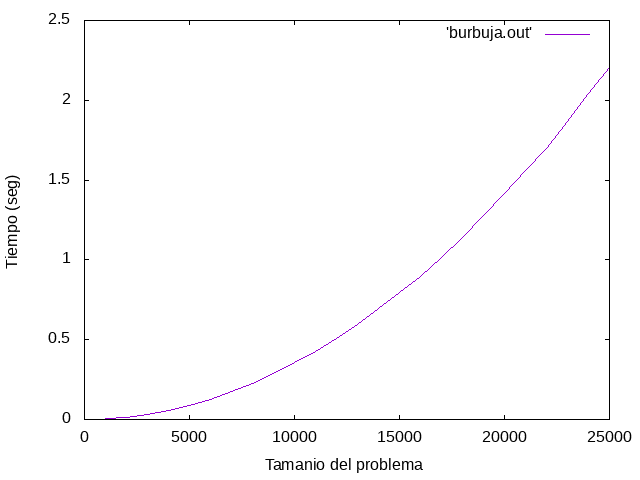
\includegraphics[scale=0.75]{empirica_burbuja.png}
\caption{Algoritmo burbuja}
\end{figure}

\begin{figure}[H]
\centering
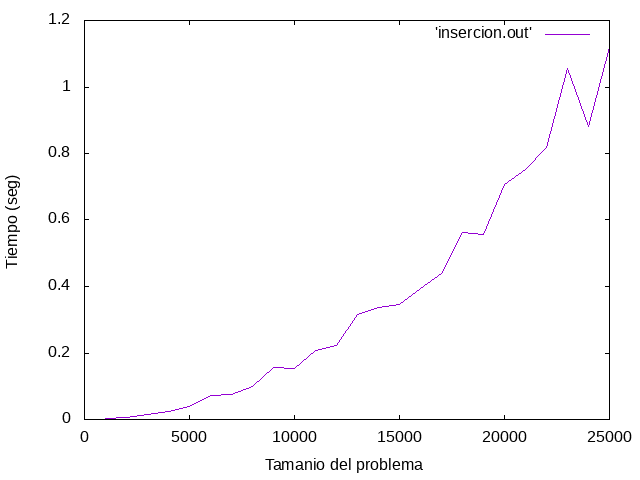
\includegraphics[scale=0.75]{empirica_insercion.png}
\caption{Algoritmo de inserción}
\end{figure}

\begin{figure}[H]
\centering
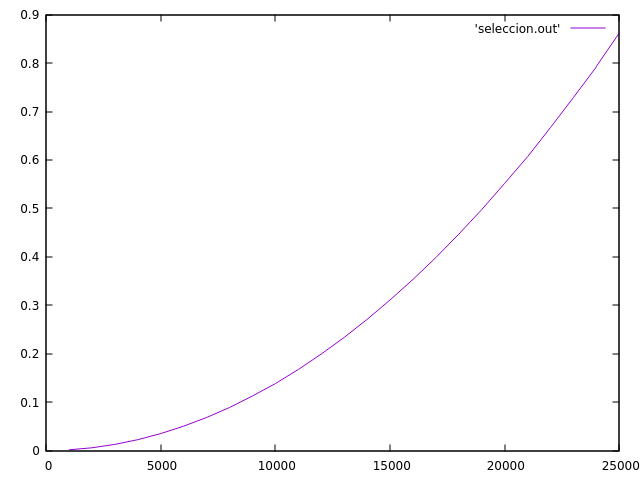
\includegraphics[scale=0.75]{empirica_seleccion.png}
\caption{Algoritmo de selección}
\end{figure}
\subsubsection{Algoritmo con eficiencia $O(n^3)$}
\begin{figure}[H]
\centering
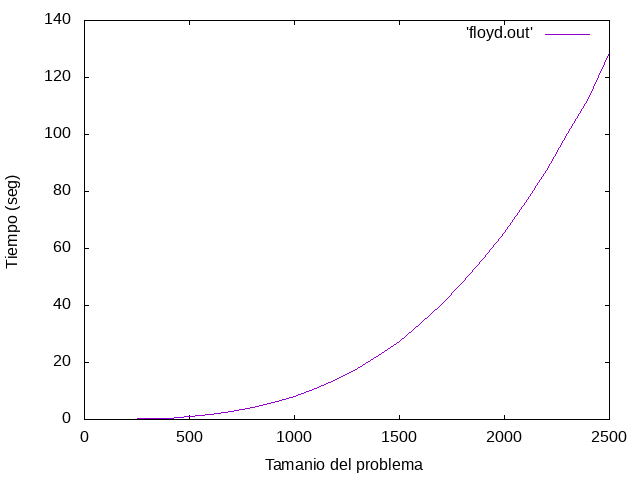
\includegraphics[scale=0.75]{empirica_floyd.png}
\caption{Algoritmo de Floyd}
\end{figure}

\subsubsection{Algoritmos con eficiencia $O(n \cdot log(n))$}

\begin{figure}[H]
\centering
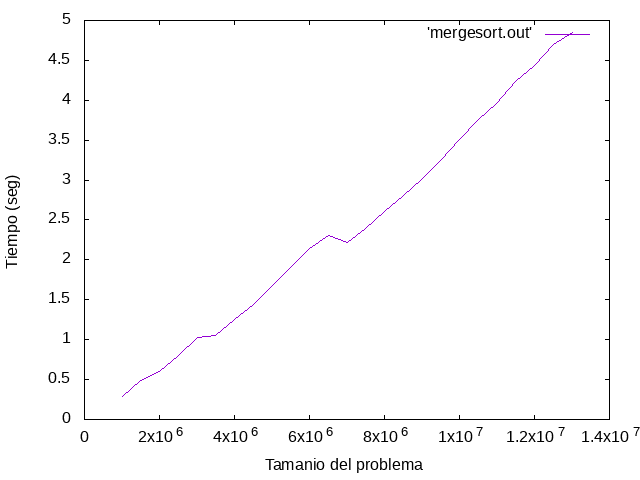
\includegraphics[scale=0.75]{empirica_mergesort.png}
\caption{Algoritmo mergesort}
\end{figure}

\begin{figure}[H]
\centering
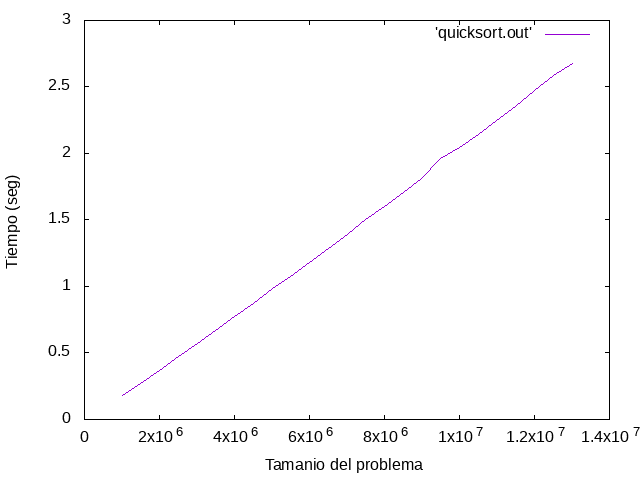
\includegraphics[scale=0.75]{empirica_quicksort.png}
\caption{Algoritmo quicksort}
\end{figure}

\begin{figure}[H]
\centering
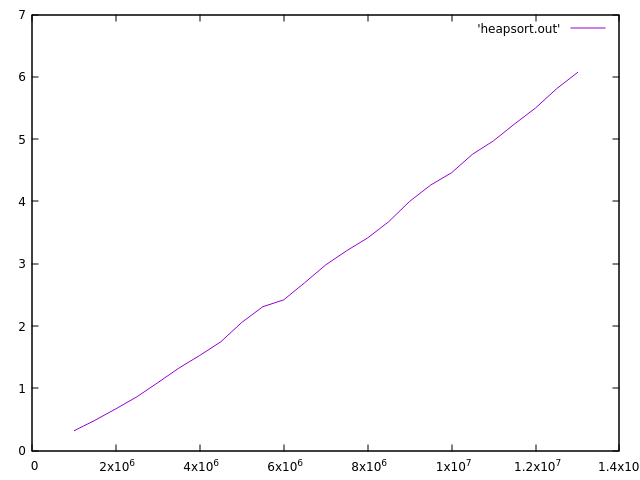
\includegraphics[scale=0.75]{empirica_heapsort.png}
\caption{Algoritmo heapsort}
\end{figure}

\subsubsection{Algoritmo con eficiencia $O(2^n)$}

\begin{figure}[H]
\centering
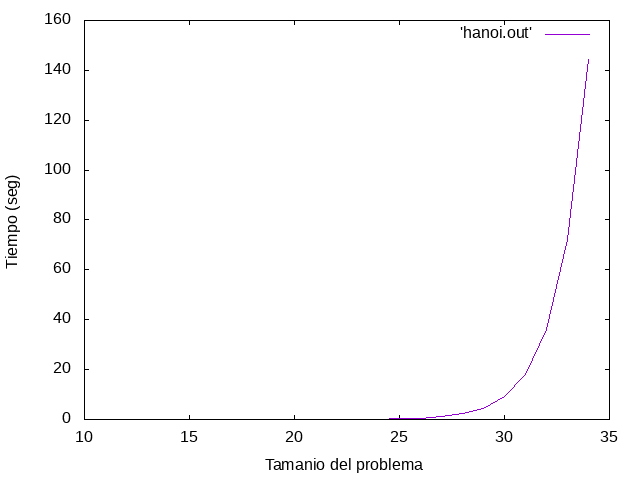
\includegraphics[scale=0.75]{empirica_hanoi.png}
\caption{Algoritmo Hanoi}
\end{figure}

\subsubsection{Comparación entre algoritmos de ordenación}
A simple vista solo podremos ver el trabajo de los algoritmos rápidos (\textit{heapsort}, \textit{mergesort} y \textit{quicksort}), ya que trabajan con tamaños de problema muy superiores al resto de algoritmos.

\begin{figure}[H]
\centering
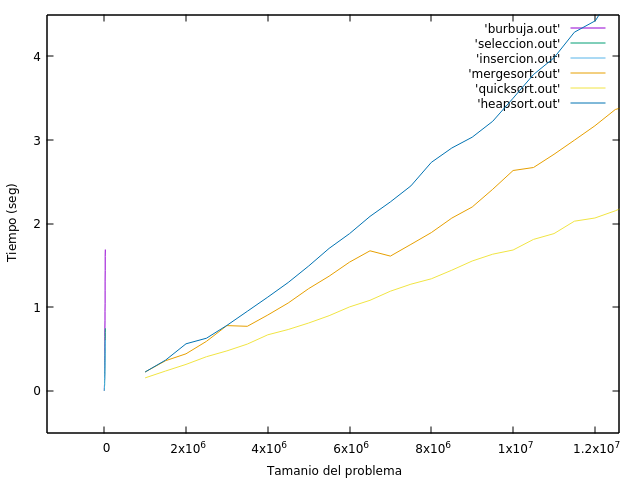
\includegraphics[scale=0.75]{empirica_ordenacion_comparacion.png}
\caption{Comparación de algoritmos de ordenación}
\end{figure}

Si hacemos zoom, podremos ver mejor la diferencia:

\begin{figure}[H]
\centering
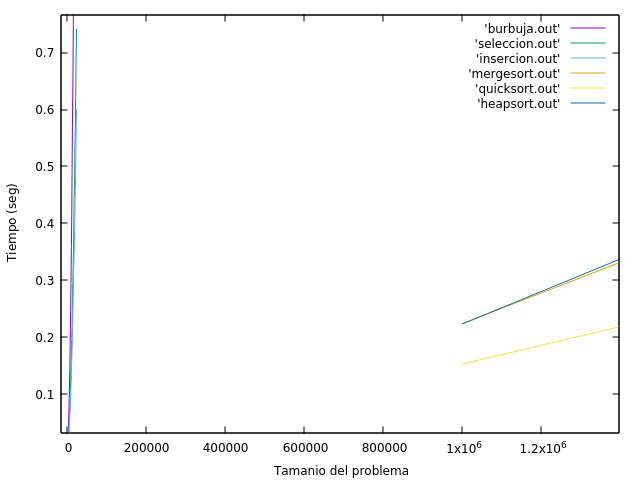
\includegraphics[scale=0.75]{empirica_ordenacion_comparacion_zoom.png}
\caption{Comparación de algoritmos de ordenación (zoom)}
\end{figure}
\subsection{Variación de la eficiencia empírica}
\label{sec:variacion}
En esta sección demostraremos empíricamente el \emph{Principio de invarianza}.
\begin{ppio}[de Invarianza]
Dos implementaciones diferentes de un  mismo  algoritmo  no  difieren  en  eficiencia  más  que,  a  lo  sumo,  en  una constante multiplicativa.
\end{ppio}
Para ello, ejecutaremos los algoritmos en una arquitectura distinta, el \textit{\nameref{sec:pc2}}.
Comenzamos con una tabla donde podremos observar la constante en cuestión según el tiempo medio de ejecución de cada algoritmo:
\begin{table}[H]
\centering
\begin{tabular}{|c|c|c|c|}
\hline
\textbf{Algoritmo} & \textbf{Tiempo medio PC 1} & \textbf{Tiempo medio PC 2} & \textbf{Constante} \\
\hline
Burbuja & pc1 & pc2 & cte\\
\hline
Inserción & pc1 & pc2 & cte\\
\hline
Selección & pc1 & pc2 & cte\\
\hline
Mergesort & pc1 & pc2 & cte\\
\hline
Quicksort & pc1 & pc2 & cte\\
\hline
Heapsort & pc1 & pc2 & cte\\
\hline
Floyd & pc1 & pc2 & cte\\
\hline
Hanoi & pc1 & pc2 & cte\\
\hline
\end{tabular}
\caption{Comparación entre ambos entornos de ejecución}
\end{table}
\subsubsection{Algoritmos con eficiencia $O(n^2)$}
\begin{figure}[H]
\centering
\begin{subfigure}[b]{0.45\textwidth}
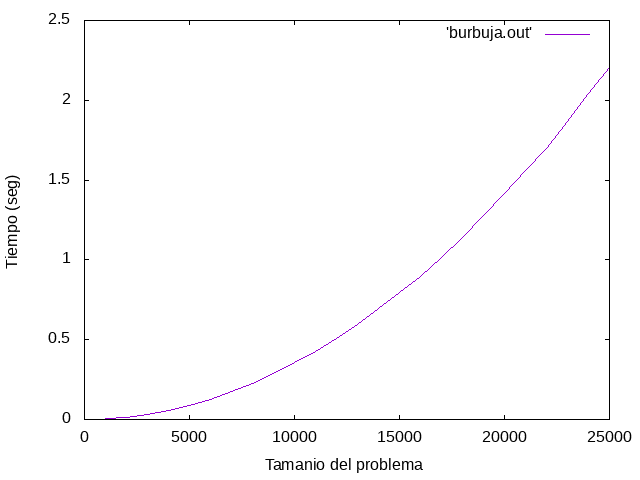
\includegraphics[scale=0.45]{empirica_burbuja.png}
\caption{\nameref{sec:pc1}}
\end{subfigure}
\quad
\begin{subfigure}[b]{0.45\textwidth}
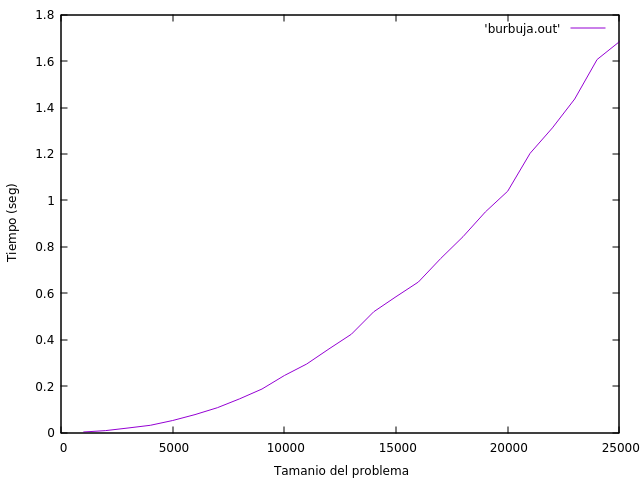
\includegraphics[scale=0.45]{empirica_burbuja_2.png}
\caption{\nameref{sec:pc2}}
\end{subfigure}
\begin{tabular}{|c|c|c|}
\hline
\textbf{Tamaño} & \textbf{Tiempo PC 1} & \textbf{Tiempo PC 2} \\
\hline
t & t1 & t2 \\
\hline
\end{tabular}
\caption{Algoritmo burbuja}
\end{figure}

\begin{figure}[H]
\centering
\begin{subfigure}[b]{0.45\textwidth}
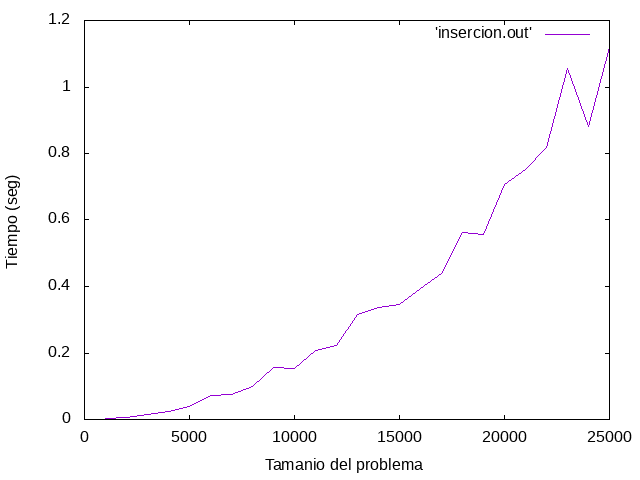
\includegraphics[scale=0.45]{empirica_insercion.png}
\caption{\nameref{sec:pc1}}
\end{subfigure}
\quad
\begin{subfigure}[b]{0.45\textwidth}
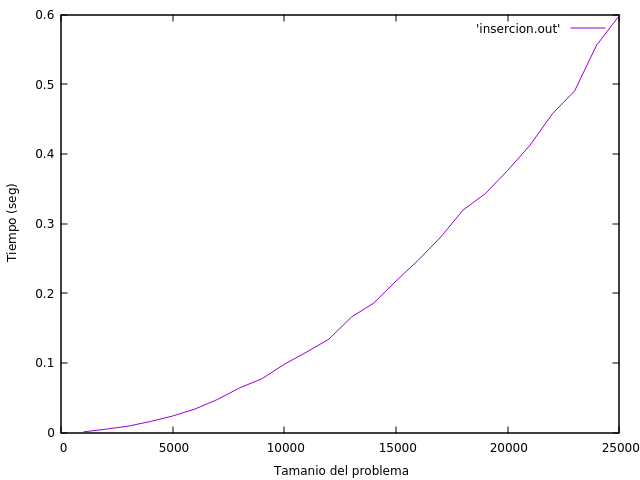
\includegraphics[scale=0.45]{empirica_insercion_2.png}
\caption{\nameref{sec:pc2}}
\end{subfigure}
\begin{tabular}{|c|c|c|}
\hline
\textbf{Tamaño} & \textbf{Tiempo PC 1} & \textbf{Tiempo PC 2} \\
\hline
t & t1 & t2 \\
\hline
\end{tabular}
\caption{Algoritmo de inserción}
\end{figure}

\begin{figure}[H]
\centering
\begin{subfigure}[b]{0.45\textwidth}
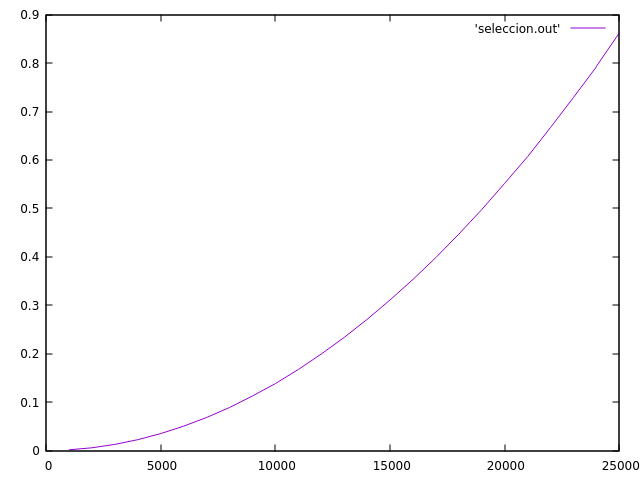
\includegraphics[scale=0.45]{empirica_seleccion.png}
\caption{\nameref{sec:pc1}}
\end{subfigure}
\quad
\begin{subfigure}[b]{0.45\textwidth}
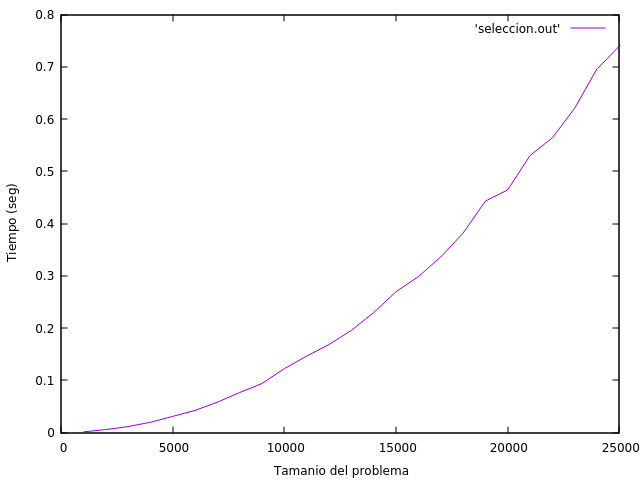
\includegraphics[scale=0.45]{empirica_seleccion_2.png}
\caption{\nameref{sec:pc2}}
\end{subfigure}
\caption{Algoritmo de selección}
\end{figure}
\subsubsection{Algoritmos con eficiencia $O(n^3)$}

\begin{figure}[H]
\centering
\begin{subfigure}[b]{0.45\textwidth}
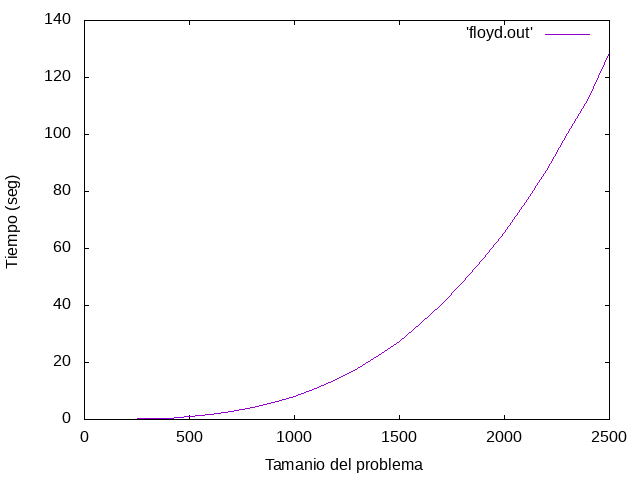
\includegraphics[scale=0.45]{empirica_floyd.png}
\caption{\nameref{sec:pc1}}
\end{subfigure}
\quad
\begin{subfigure}[b]{0.45\textwidth}
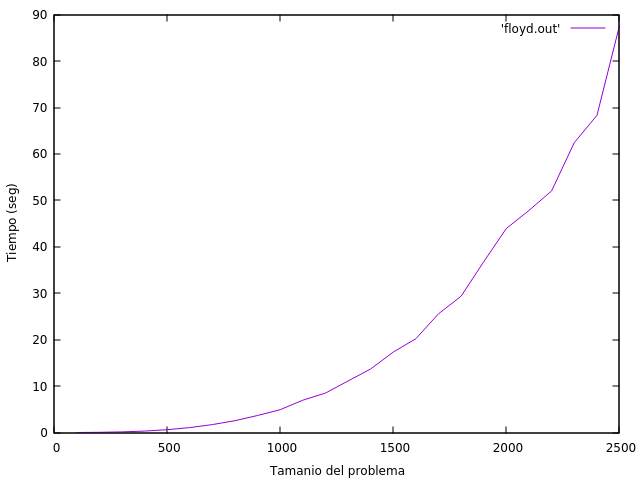
\includegraphics[scale=0.45]{empirica_floyd_2.png}
\caption{\nameref{sec:pc2}}
\end{subfigure}
\begin{tabular}{|c|c|c|}
\hline
\textbf{Tamaño} & \textbf{Tiempo PC 1} & \textbf{Tiempo PC 2} \\
\hline
t & t1 & t2 \\
\hline
\end{tabular}
\caption{Algoritmo de Floyd}
\end{figure}

\subsubsection{Algoritmos con eficiencia $O(n \cdot log(n))$}

\begin{figure}[H]
\centering
\begin{subfigure}[b]{0.45\textwidth}
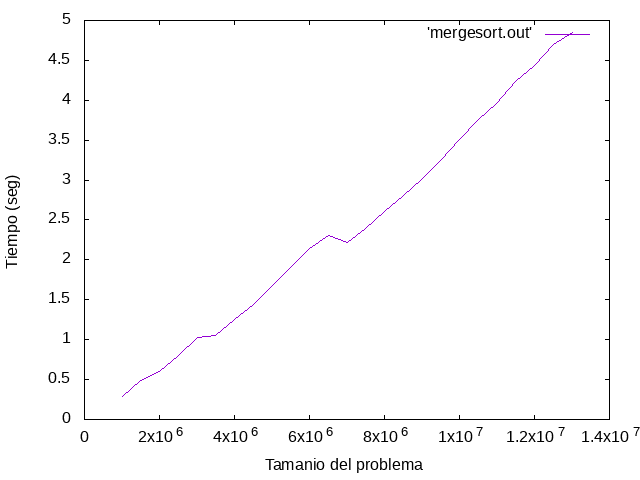
\includegraphics[scale=0.45]{empirica_mergesort.png}
\caption{\nameref{sec:pc1}}
\end{subfigure}
\quad
\begin{subfigure}[b]{0.45\textwidth}
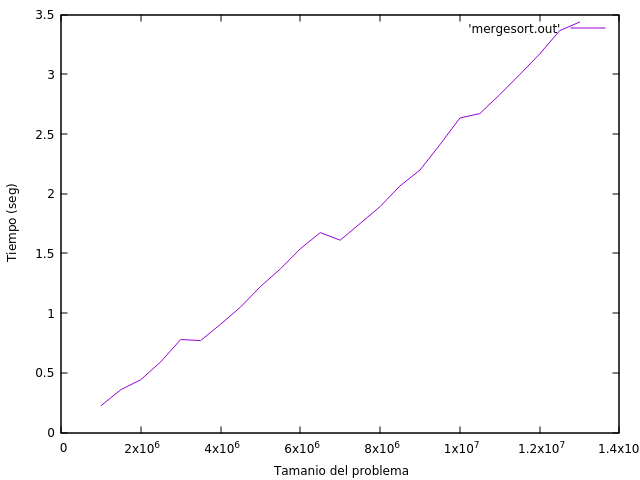
\includegraphics[scale=0.45]{empirica_mergesort_2.png}
\caption{\nameref{sec:pc2}}
\end{subfigure}
\begin{tabular}{|c|c|c|}
\hline
\textbf{Tamaño} & \textbf{Tiempo PC 1} & \textbf{Tiempo PC 2} \\
\hline
t & t1 & t2 \\
\hline
\end{tabular}
\caption{Algoritmo mergesort}
\end{figure}

\begin{figure}[H]
\centering
\begin{subfigure}[b]{0.45\textwidth}
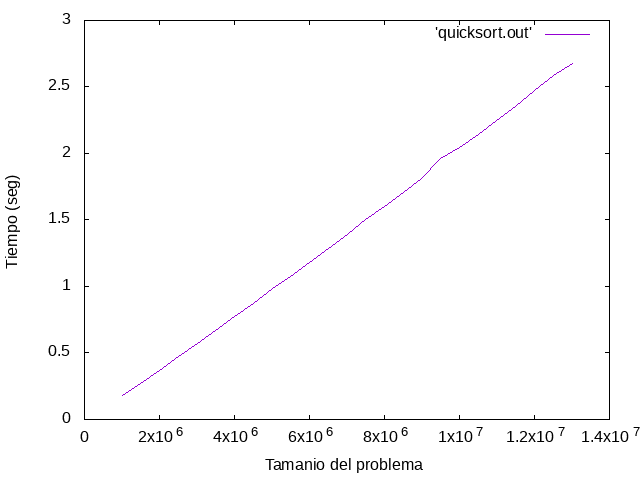
\includegraphics[scale=0.45]{empirica_quicksort.png}
\caption{\nameref{sec:pc1}}
\end{subfigure}
\quad
\begin{subfigure}[b]{0.45\textwidth}
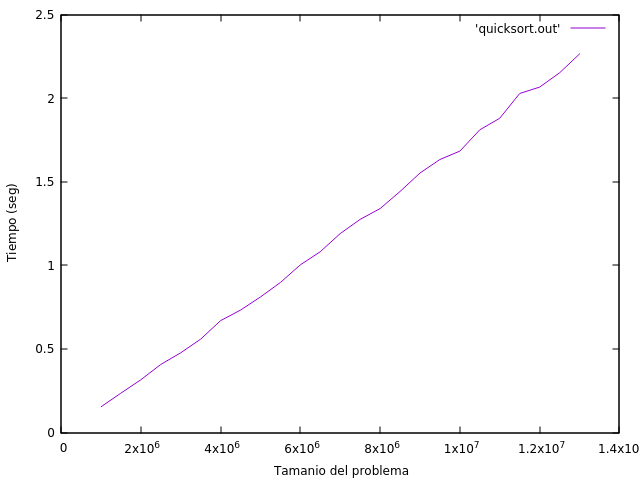
\includegraphics[scale=0.45]{empirica_quicksort_2.png}
\caption{\nameref{sec:pc2}}
\end{subfigure}
\begin{tabular}{|c|c|c|}
\hline
\textbf{Tamaño} & \textbf{Tiempo PC 1} & \textbf{Tiempo PC 2} \\
\hline
t & t1 & t2 \\
\hline
\end{tabular}
\caption{Algoritmo quicksort}
\end{figure}

\begin{figure}[H]
\centering
\begin{subfigure}[b]{0.45\textwidth}
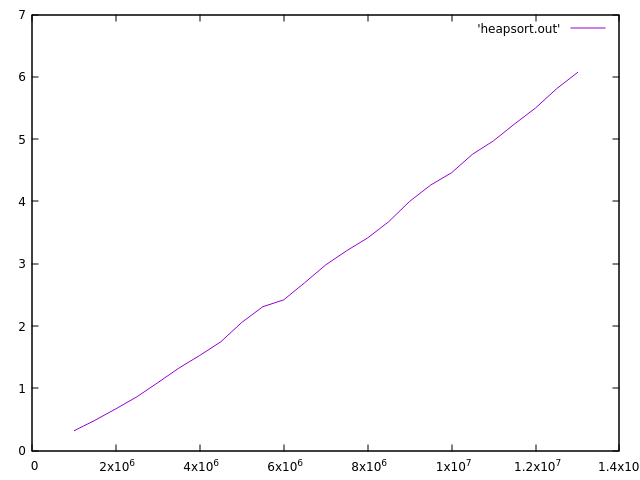
\includegraphics[scale=0.45]{empirica_heapsort.png}
\caption{\nameref{sec:pc1}}
\end{subfigure}
\quad
\begin{subfigure}[b]{0.45\textwidth}
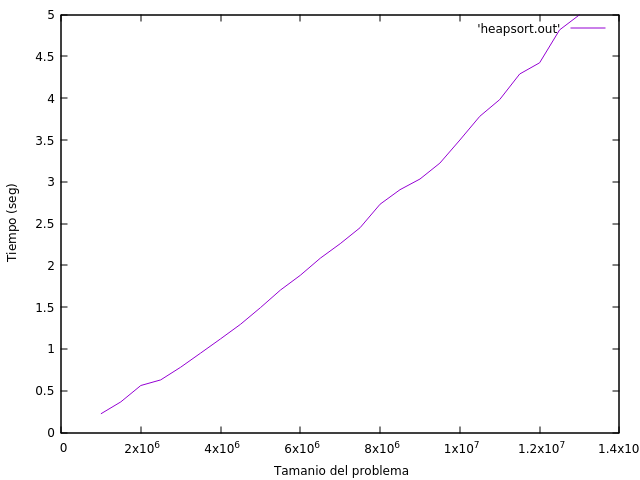
\includegraphics[scale=0.45]{empirica_heapsort_2.png}
\caption{\nameref{sec:pc2}}
\end{subfigure}
\begin{tabular}{|c|c|c|}
\hline
\textbf{Tamaño} & \textbf{Tiempo PC 1} & \textbf{Tiempo PC 2} \\
\hline
t & t1 & t2 \\
\hline
\end{tabular}
\caption{Algoritmo heapsort}
\end{figure}

\subsubsection{Algoritmo con eficiencia $O(2^n)$}

\begin{figure}[H]
\centering
\begin{subfigure}[b]{0.45\textwidth}
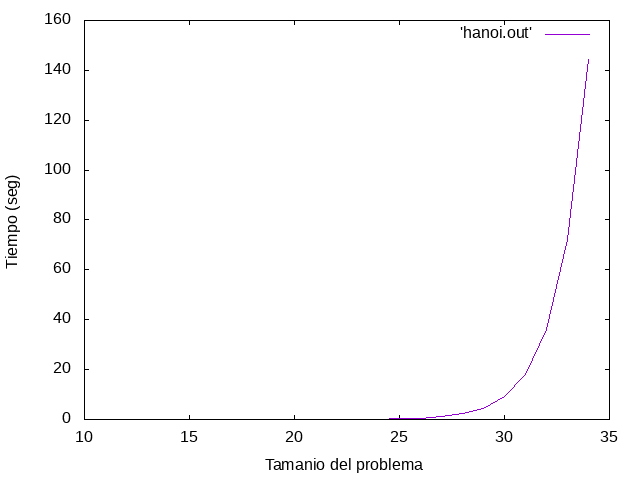
\includegraphics[scale=0.45]{empirica_hanoi.png}
\caption{\nameref{sec:pc1}}
\end{subfigure}
\quad
\begin{subfigure}[b]{0.45\textwidth}
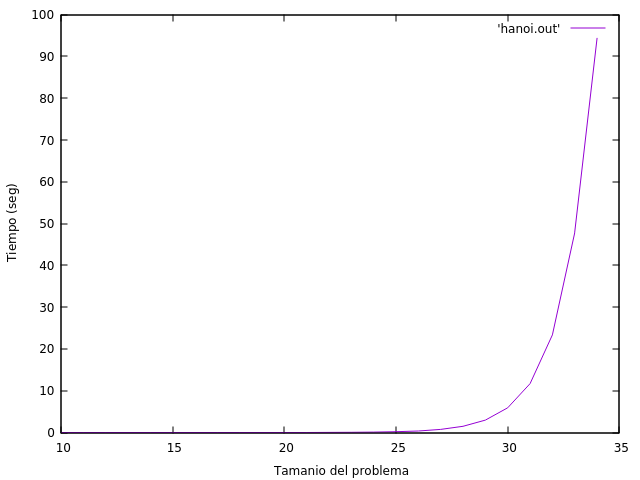
\includegraphics[scale=0.45]{empirica_hanoi_2.png}
\caption{\nameref{sec:pc2}}
\end{subfigure}
\begin{tabular}{|c|c|c|}
\hline
\textbf{Tamaño} & \textbf{Tiempo PC 1} & \textbf{Tiempo PC 2} \\
\hline
t & t1 & t2 \\
\hline
\end{tabular}
\caption{Algoritmo de Hanoi}
\end{figure}

\subsubsection{Algoritmos con eficiencia $O(n \cdot log(n))$}

\section{Cálculo de la eficiencia híbrida}

\subsubsection{Algoritmos con eficiencia $O(n^2)$}

\subsubsection{Algoritmos con eficiencia $O(n^3)$}

\subsubsection{Algoritmos con eficiencia $O(n \cdot log(n))$}

\subsubsection{Algoritmo con eficiencia $O(2^n)$}

\subsubsection{Algoritmos con eficiencia $O(n \cdot log(n))$}

%%%%%%%%%%%%%%%%%%%%%%%%%%%%Fin del documento%%%%%%%%%%%%%%%%%%%%%%%%%%%%%%%%
\end{document}
